\section{Boundary conformal neural fields}
\label{sec:boundary}

A boundary relates the two chiral sectors and retains a single conformal
algebra.  For the upper half-plane
$\mathbb H=\{z\in\mathbb C:\operatorname{Im}z>0\}$, the free-field
boundary conditions can be imposed directly on the neural features by
reflection.  This gives an explicit realization of boundary neural fields,
complementary to the embedding-space defect construction of
\cite{Capuozzo:2025ozt}.  We first impose the boundary condition at finite
width and then identify the conformal gluing of the limiting free fields
\cite{Cardy:2004hm}.

\subsection{Reflected scalar features}

Using the \emph{same} momenta and phases at a point and its image, define
\begin{equation}
\Phi_{\sigma,N}(z,\bar z)
=\frac{\phi_N(z,\bar z)+\sigma\phi_N(\bar z,z)}{\sqrt2},
\qquad \sigma\in\{+1,-1\}.
\label{eq:boundary-scalar-features}
\end{equation}
Here $\phi_N(\bar z,z)$ means evaluation of the real Fourier field at
$(x,-y)$.  Reflection makes $\Phi_{+,N}$ even and $\Phi_{-,N}$ odd in
$y$, so every realization satisfies
\begin{equation}
\left.\partial_y\Phi_{+,N}\right|_{y=0}=0,
\qquad
\left.\Phi_{-,N}\right|_{y=0}=0.
\label{eq:boundary-exact-bcs}
\end{equation}
These are respectively Neumann and homogeneous Dirichlet conditions.
Independent draws at the two reflected points would not satisfy these
identities.  The factor $1/\sqrt2$ preserves the normalization of the
direct bulk singularity.

The isotropic ensemble covariance obeys the image formula at every width
and finite spectral cutoff:
\begin{equation}
K^\sigma_{\Lambda,\tau}(z,w)
=K_{\Lambda,\tau}(z-w)
+\sigma K_{\Lambda,\tau}(z-\bar w).
\label{eq:boundary-regulated-kernel}
\end{equation}
This follows by expanding the four terms in
$\mathbb E[\Phi_{\sigma,N}(z)\Phi_{\sigma,N}(w)]$ and using reflection
invariance of the momentum law.  For a fixed sampled momentum set, the
conditional covariance instead retains all four terms; reflection
invariance is an ensemble property.  On separated points in the scaling
window, the limiting image kernel is
\begin{equation}
K^\sigma(z,w)
=-\log|z-w|^2-\sigma\log|z-\bar w|^2,
\label{eq:boundary-log-kernel}
\end{equation}
modulo the scalar infrared constant.  This constant cancels for Dirichlet
conditions and is removed by taking covariance differences for Neumann
conditions.  At fixed regulator, infinite width gives the Gaussian field
with covariance \eqref{eq:boundary-regulated-kernel}; removal of the
regulator is still needed for the conformal kernel.

The reflected construction also fixes the current gluing.  With
$J_{\sigma,N}=i\partial\Phi_{\sigma,N}$ and
$\bar J_{\sigma,N}=i\bar\partial\Phi_{\sigma,N}$, where the bar labels
right chirality, the boundary derivatives give
\begin{equation}
\left.J_{\sigma,N}\right|_{\mathbb R}
=\left.\sigma\bar J_{\sigma,N}\right|_{\mathbb R}.
\label{eq:boundary-current-gluing}
\end{equation}
This identity is exact even though the regulated currents are not
holomorphic.  In the limiting free-field representation, normal ordering
with the corresponding reflected contractions gives
\begin{equation}
\left.T^B\right|_{\mathbb R}
=\left.\bar T^B\right|_{\mathbb R},
\qquad T^B=\tfrac12:JJ:.
\label{eq:boundary-stress-gluing}
\end{equation}
The doubled stress tensor then defines one Virasoro algebra with $c=1$.
Equivalently, in the closed-channel boundary-state convention the local
condition is $(L_n-\bar L_{-n})|B\rangle=0$
\cite{Cardy:2004hm}.  This stress-tensor gluing condition is distinct from
the annulus consistency conditions on a physical boundary state.

\subsection{Doubled fermions and superconformal gluing}

Let $\chi$ be the doubled chiral Majorana field obtained from the admissible
CAR construction of section~\ref{sec:susy}.  A reflecting boundary is
specified by
\begin{equation}
\psi_L(z)=\chi(z),\qquad
\psi_R(\bar z)=\eta\chi(\bar z),\qquad \eta=\pm1.
\label{eq:boundary-doubled-fermion}
\end{equation}
Thus $\psi_L(x)=\eta\psi_R(x)$ on the real axis.  At finite feature
width this relation can be imposed separately on the positive- and
negative-frequency features in
\eqref{eq:random-cauchy-fermions}: the right sector evaluates the same mode
indices and Berezin pairs at the reflected argument, with the factor
$\eta$.  The reflection relation is then exact for each ordered feature
field.  Convergence of its contractions and admissibility of the retained
CAR pairing remain the conditions described in section~\ref{sec:susy}.

The continuum two-point functions form a matrix, with rows and columns
ordered as $(L,R)$:
\begin{equation}
S_\eta(z,w)=
\begin{pmatrix}
\displaystyle\frac1{z-w}&\displaystyle\frac{\eta}{z-\bar w}\\[6pt]
\displaystyle\frac{\eta}{\bar z-w}&
\displaystyle\frac1{\bar z-\bar w}
\end{pmatrix}.
\label{eq:boundary-fermion-matrix}
\end{equation}
In particular, the image term belongs to the mixed-chirality contraction.
The matrix satisfies $S_{ab}(z,w)=-S_{ba}(w,z)$, including the fermionic
exchange sign.  Treating $1/(z-w)+\eta/(z-\bar w)$ as a single identical
fermion two-point function would not have this exchange property.

For the independent free boson and fermion, set
\begin{equation}
T=T^B-\tfrac12:\psi_L\partial\psi_L:,
\qquad G=:J\psi_L:,
\label{eq:boundary-supercurrent}
\end{equation}
and define the right fields with the same phase conventions.  The two
reflection signs give
\begin{equation}
\left.T\right|_{\mathbb R}=\left.\bar T\right|_{\mathbb R},
\qquad
\left.G\right|_{\mathbb R}
=\left.\rho\bar G\right|_{\mathbb R},
\qquad \rho=\sigma\eta.
\label{eq:boundary-superconformal-gluing}
\end{equation}
Both $\rho=+1$ and $\rho=-1$ specify a preserved boundary
$\CN=1$ superconformal algebra with $c=3/2$
\cite{Gaberdiel:2008gk}.  In the convention $G=\bar G$, one chooses
$\eta=\sigma$; the opposite relative sign selects the other preserved
supercharge.  The reflection sign $\eta$ is separate from the choice of
NS or Ramond periodicity on a cylinder.  The present construction uses the
NS modes of section~\ref{sec:susy}.

The mixed contractions of the limiting fields make this gluing explicit:
\begin{equation}
\langle J(z)\bar J(\bar w)\rangle=\frac{\sigma}{(z-\bar w)^2},
\qquad
\langle G(z)\bar G(\bar w)\rangle
=\frac{\sigma\eta}{(z-\bar w)^3}.
\label{eq:boundary-mixed-current-kernels}
\end{equation}
The second relation follows by Wick factorization of the independent
sectors.  A numerical product of their two-point estimates consequently
does not supply an independent measurement of a supersymmetry Ward
identity.

\subsection{Boundary correlations}

The image construction has observables that resolve the distance to the
boundary.  For the scalar, subtracting variances at two heights cancels the
bulk coincident term:
\begin{align}
V_\sigma(y;y_0)
&:=\mathbb E[\Phi_{\sigma,N}(iy)^2]
-\mathbb E[\Phi_{\sigma,N}(iy_0)^2]\nonumber\\
&=\sigma\bigl[K_{\Lambda,\tau}(2iy)
-K_{\Lambda,\tau}(2iy_0)\bigr]
\longrightarrow -2\sigma\log(y/y_0).
\label{eq:boundary-height-statistic}
\end{align}
The logarithmic slope is $-2\sigma$ in the normalization
$K=-\log|z-w|^2$ used throughout this paper.  For Neumann conditions,
figure~\ref{fig:boundary-kernels}(a) compares this prediction with the
regulated kernel and phase-averaged feature estimates.  The slope from 32
independent frequency batches is $-1.991\pm0.008$ (one standard error),
using $N=16\,384$ features per batch.  The matching finite-cutoff kernel has
slope $-1.999995$ over the same heights.  These error bars describe frequency
sampling after phase averaging.

For the fermion, take $z=x+i\varepsilon$ and $w=i\varepsilon$.  The mixed
correlator is
\begin{equation}
S_{LR}(z,w)=\frac{\eta}{x+2i\varepsilon},\qquad
|S_{LR}(z,w)|=\frac1{\sqrt{x^2+4\varepsilon^2}}.
\label{eq:boundary-fermion-geometry}
\end{equation}
Its magnitude approaches $1/|x|$ only for $|x|\gg2\varepsilon$; at
shorter horizontal separation the image distance resolves the height.
Figure~\ref{fig:boundary-kernels}(b) displays this crossover and its
deterministic finite-Cauchy representation.  The 32-term series differs
from the continuum mixed kernel by less than $6.6\times10^{-12}$ in
relative magnitude over the displayed points.  This is a truncation check,
separate from a random-feature sampling test.

\begin{figure}[t]
\centering
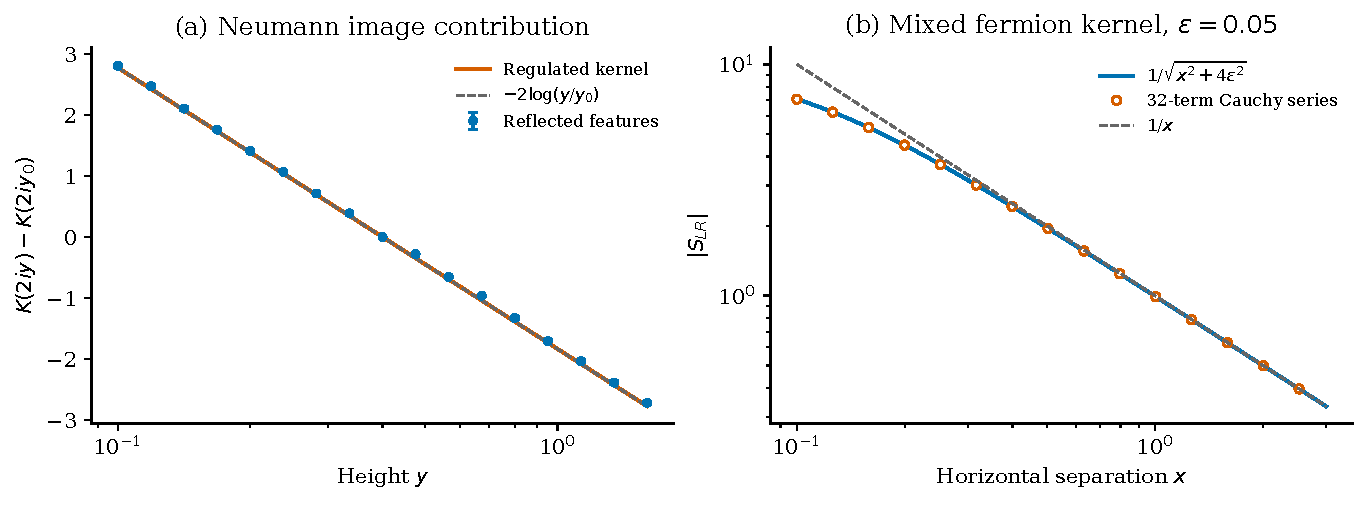
\includegraphics[width=\textwidth]{evidence/figures/boundary_kernels.pdf}
\caption{Boundary kernels from reflection.  (a) Neumann variance
differences relative to $y_0=0.4$, with the scalar bulk coincident term
removed.  Points are phase-averaged estimates from 32 independent batches
of $16\,384$ momenta; bars give one standard error of the batch mean.
The solid line uses the raised-cosine regulator with
$(\Lambda_{\rm IR},\Lambda_{\rm UV},\tau)=(10^{-3},10^3,0.15)$; the
dashed line is the continuum logarithm.  (b) Magnitude of the mixed
fermion kernel at height $\varepsilon=0.05$.  The markers evaluate a
32-term Cauchy series, the solid line is the exact image kernel, and the
dashed line is its large-separation asymptote.  Numerical methods are
given in appendix~\ref{app:boundary-methods}.}
\label{fig:boundary-kernels}
\end{figure}

These constructions establish exact feature-level boundary constraints
and the local gluing of their limiting free-field kernels and admissible
operator representations.  The finite-regulator neural measure is still
subject to the bulk reconstruction questions discussed below.  Normalized
boundary states, their zero-mode content, and annulus sewing consistency
require additional data beyond the image two-point functions.
